In the first experiment, we investigate the impact of three different dead-end handling strategies on the Gini coefficient of PageRank values across various types of graphs. In the second experiment, we attempt six different deterministic heuristics for adding edges to the graph for minimization of Gini coefficient of PageRank values. Dataset for the experiments are obtained from the \href{https://sparse.tamu.edu}{\textit{SuiteSparse Matrix Collection}} \cite{suite19}. Our experiments are reproducible. The codebase is available at our repository.\footnote{https://github.com/puzzlef/pagerank-minimize-inequality}




\subsubsection{Results}

Results, shown in Figures \ref{fig:de-gini} and \ref{fig:de-lorenz-all}, indicate that web graphs in general (except \verb|web-NotreDame|) have high Gini coefficient (i.e., high inequality) along with a social network \verb|soc-Epinions1|, and a citation network \verb|cit-Patents|. Road networks are observed to have the lowest Gini coefficient (i.e., low inequality) among all graph classes. If we take a look at the average Lorenz curve of all graphs, we observe that $50\%$ of popularity (ranks) is owned by $\approx20\%$ of the vertices. However, on the web-Stanford graph $50\%$ of popularity is owned by only $\approx3\%$ of vertices, and on the \verb|arabic-2005| (another web graph) is owned by only $\approx1\%$ of the vertices. This would be a significantly worrying level of inequality if each vertex represented a unique person. However, it is possible that many low-ranked pages are low-effort ones and thus have a high page-to-person ratio.

On the social network \verb|soc-Epinions1|, $50\%$ of popularity is owned by only $\approx7\%$ of vertices (Gini coefficient of $\approx0.66$), but on the \verb|wiki-Talk| (a communication graph) $50\%$ of popularity is owned by $\approx46\%$ of vertices (Gini coefficient of $\approx0.07$). This is quite interesting, given that wiki users are usually not ranked, while search engines always rank web pages. Road networks, such as \verb|germany_osm|, are observed to have have a distribution similar to that of \verb|wiki-Talk|.
% Future work could focus on studying the variation of the Lorenz curve and Gini coefficient of various graphs over time.




\subsection{Heuristics for Inequality minimization}

In this experiment we study the minimization of Gini coefficient of PageRank values on a number of graphs, using six different deterministic heuristics for adding edges to the graph. First, the PageRank of each vertex is computed in the original graph, and the original Gini coefficient is obtained. A heuristic is then run to obtain the most suitable edge to be added. After this edge is added, the same heuristic is run again. For each heuristic $1000$ edges are added. We plot the variation of Gini coefficient with each added edge for each heuristic.

Our first heuristic, \textbf{edgeInsertCxrx}, adds an edge between the highest contributing vertex to the lowest rank vertex. The idea behind this heuristic is to provide the highest possible increase in rank to the lowest rank vertex. We obtained the highest contributing vertex by finding the vertex with highest $R/(d+1)$ value.

The second heuristic called \textbf{edgeInsertCxSx} is based on the idea of providing the highest possible increase in rank to a vertex which directly or indirectly links to many other vertices (so that it increases the rank of a large number of other vertices as well). This is achieved by adding an edge from the highest contributing vertex to the vertex with highest reverse PageRank. Here, the reverse PageRank of a vertex is obtained by reversing (transposing) the graph, and calculating the PageRanks.

The third heuristic called \textbf{edgeInsertCxSr} is an extension of \textbf{edgeInsertCxSx}, and it prioritizes increasing the rank of vertices which link (directly or indirectly) to a large number of vertices having a low PageRank score. This is done by calculating a modified reverse PageRank, that prioritizes contribution from vertices with low forward PageRank. Here, the reverse rank of each vertex is calculated as $r_u = \alpha R_u r_v / d_v + (1-\alpha)/N$, where $r_u$ is the reverse rank of a given vertex and $R_u$ is its forward rank (precomputed), $r_v$ is the reverse rank of a target vertex and $d_v$ is its in-degree, $\alpha$ is the damping factor, and $N$ is the number of vertices in the graph.

The remaining three heuristics \textbf{edgeInsertCRrx}, \textbf{edgeInsert-CRSx}, and \textbf{edgeInsertCRSr} are a variation of the three heuristics mentioned above where the source vertex is chosen such that it minimizes the rank of the highest ranked vertex. That is, we choose the source vertex with highest contribution to the highest rank vertex. The idea is to reduce rank of high-ranked vertices and increase the rank of low-ranked vertices at the same time, thus reducing inequality.


\subsubsection{Results}

\ignore{It is observed that web graphs tend to have the highest inequality (Gini coefficient), while road networks tend to have the lowest.}As shown in Figure \ref{fig:im-all}, results indicate that the heuristics usually succeed in reducing inequality on graphs with high Gini coefficient (such as web graphs and social networks), but mostly fail on graphs with low Gini coefficient (such as road networks and collaboration networks). It is also observed that the rate of decrease in Gini coefficient decreases as more and more edges are added to graph. In general, we observe that the heuristics \textit{edgeInsertCxrx}, \textit{edgeInsertCxSx}, and \textit{edgeInsertCxSr} perform the best, with \textit{edgeInsertCxSx}, and \textit{edgeInsertCxSr} performing almost identically. \textbf{edgeInsertCxrx} and \textbf{edgeInsertCxSx} heuristics would therefore be the best choices, given that \textit{edgeInsertCxSr} requires a modified PageRank computation.

Based on these results, a suitable approach to minimizing inequality would be to apply both the \textit{edgeInsertCxrx} and \textit{edgeInsertCxSx} heuristics and choose the the best among them for each edge addition. Future research work can include exploring randomized heuristics or looking for better deterministic heuristics.

\begin{figure*}[hbtp]
  \centering
  \subfigure{
    \label{fig:im-key}
    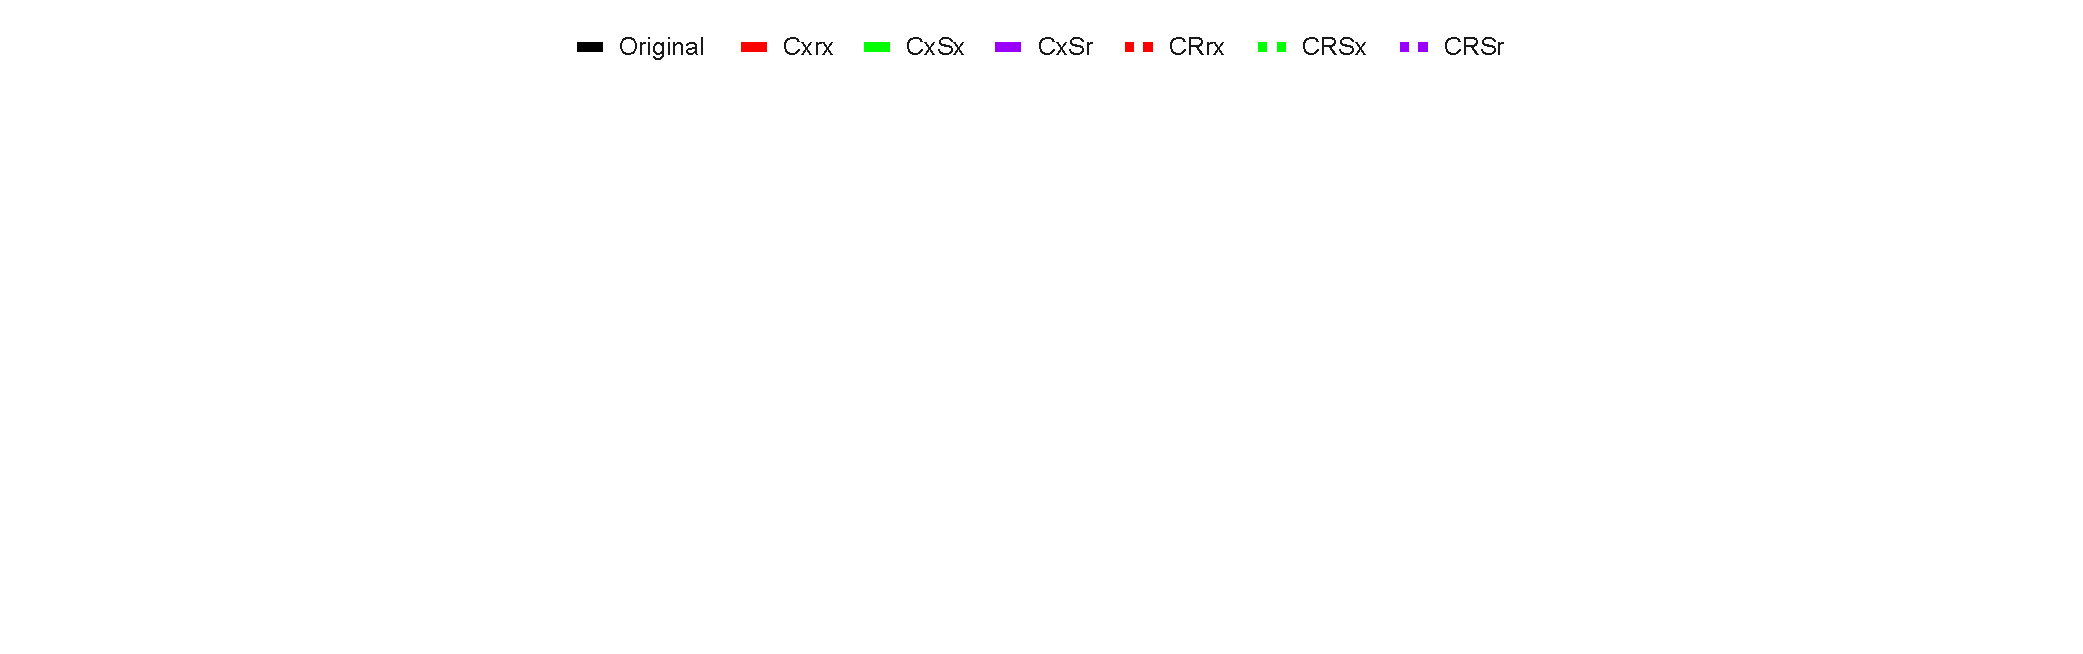
\includegraphics[width=0.98\linewidth]{out/im-key.pdf}
  } \\[-2ex]
  \subfigure{
    \label{fig:im-web-Stanford}
    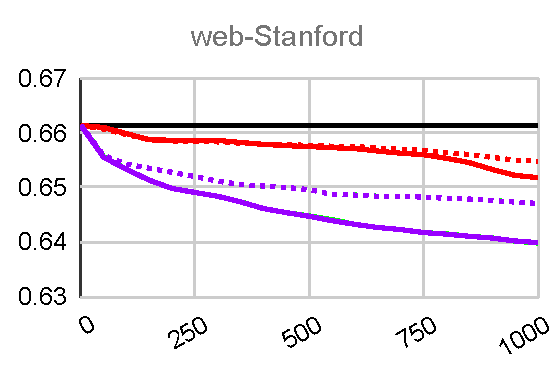
\includegraphics[width=0.23\linewidth]{out/im-web-Stanford.pdf}
  }
  \subfigure{
    \label{fig:im-web-BerkStan}
    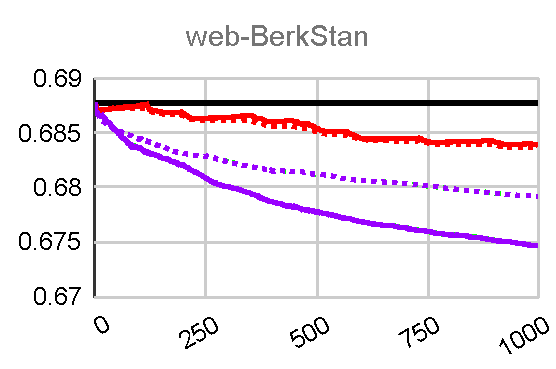
\includegraphics[width=0.23\linewidth]{out/im-web-BerkStan.pdf}
  }
  \subfigure{
    \label{fig:im-web-Google}
    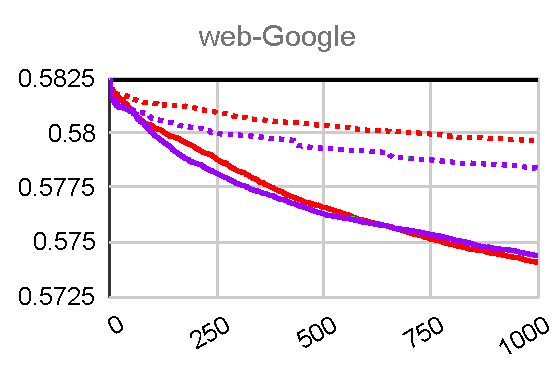
\includegraphics[width=0.23\linewidth]{out/im-web-Google.pdf}
  }
  \subfigure{
    \label{fig:im-web-NotreDame}
    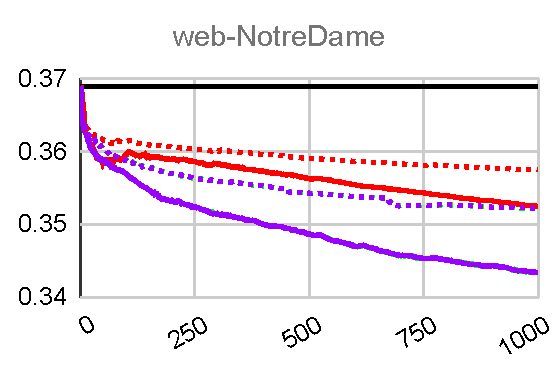
\includegraphics[width=0.23\linewidth]{out/im-web-NotreDame.pdf}
  }
  \subfigure{
    \label{fig:im-soc-Slashdot0811}
    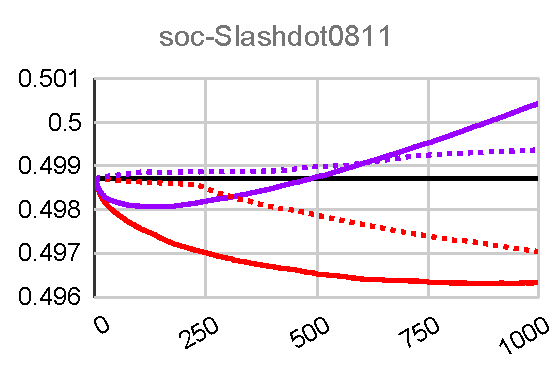
\includegraphics[width=0.23\linewidth]{out/im-soc-Slashdot0811.pdf}
  }
  \subfigure{
    \label{fig:im-soc-Slashdot0902}
    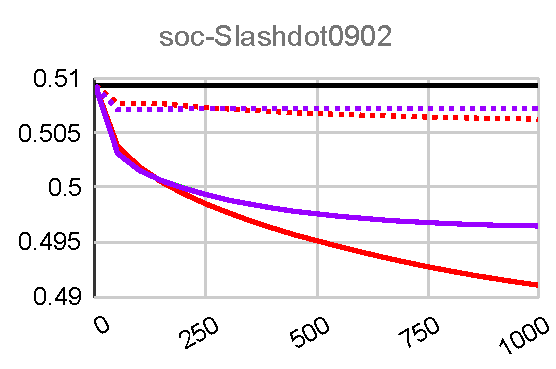
\includegraphics[width=0.23\linewidth]{out/im-soc-Slashdot0902.pdf}
  }
  \subfigure{
    \label{fig:im-soc-Epinions1}
    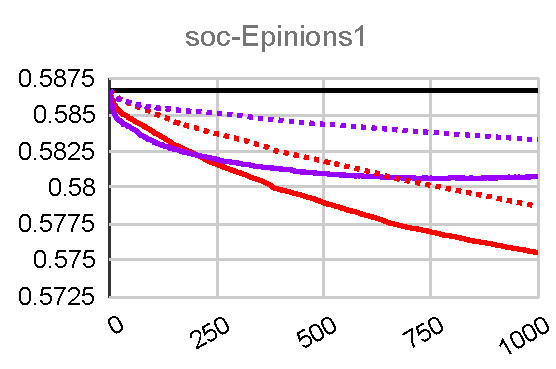
\includegraphics[width=0.23\linewidth]{out/im-soc-Epinions1.pdf}
  }
  \subfigure{
    \label{fig:im-soc-LiveJournal1}
    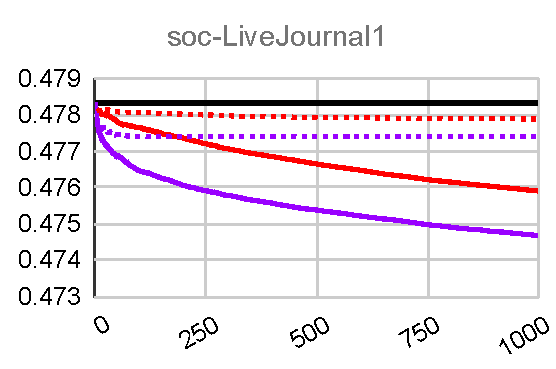
\includegraphics[width=0.23\linewidth]{out/im-soc-LiveJournal1.pdf}
  }
  \subfigure{
    \label{fig:im-coAuthorsDBLP}
    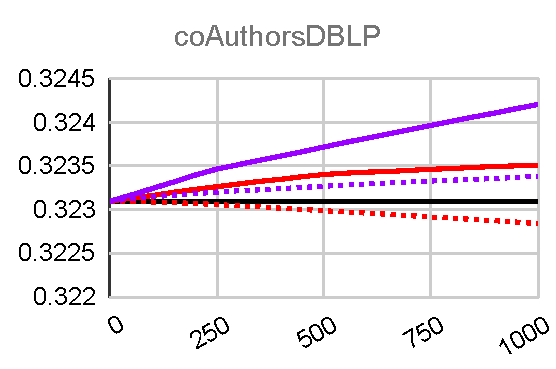
\includegraphics[width=0.23\linewidth]{out/im-coAuthorsDBLP.pdf}
  }
  \subfigure{
    \label{fig:im-coAuthorsCiteseer}
    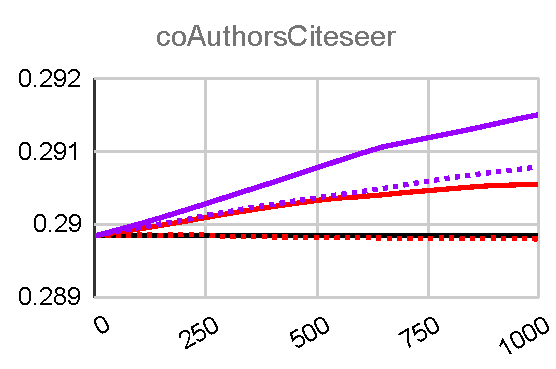
\includegraphics[width=0.23\linewidth]{out/im-coAuthorsCiteseer.pdf}
  }
  \subfigure{
    \label{fig:im-coPapersCiteseer}
    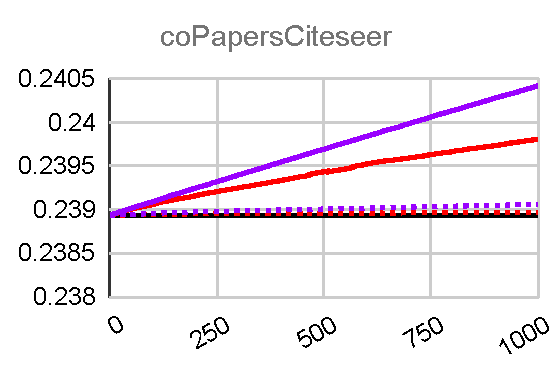
\includegraphics[width=0.23\linewidth]{out/im-coPapersCiteseer.pdf}
  }
  \subfigure{
    \label{fig:im-coPapersDBLP}
    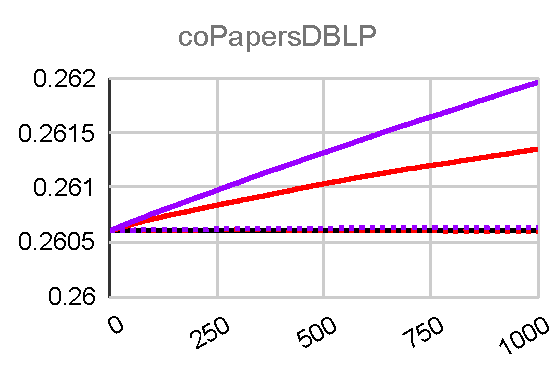
\includegraphics[width=0.23\linewidth]{out/im-coPapersDBLP.pdf}
  }
  \subfigure{
    \label{fig:im-italy_osm}
    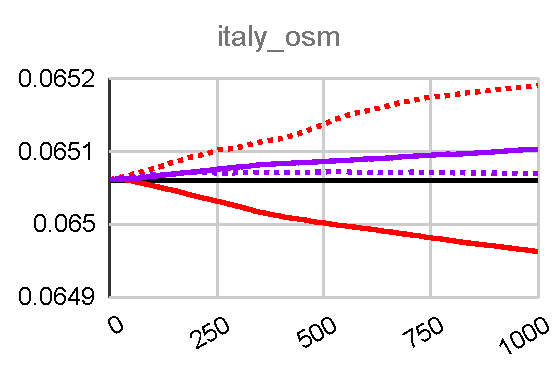
\includegraphics[width=0.23\linewidth]{out/im-italy_osm.pdf}
  }
  \subfigure{
    \label{fig:im-great-britain_osm}
    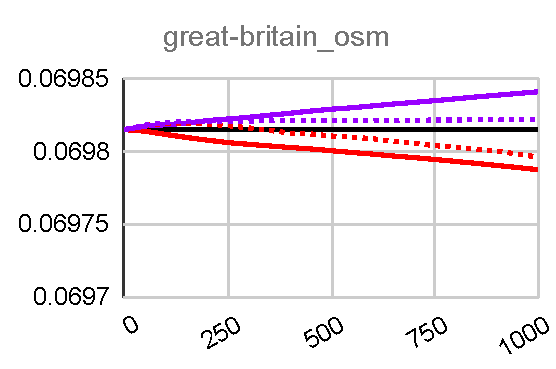
\includegraphics[width=0.23\linewidth]{out/im-great-britain_osm.pdf}
  }
  \subfigure{
    \label{fig:im-germany_osm}
    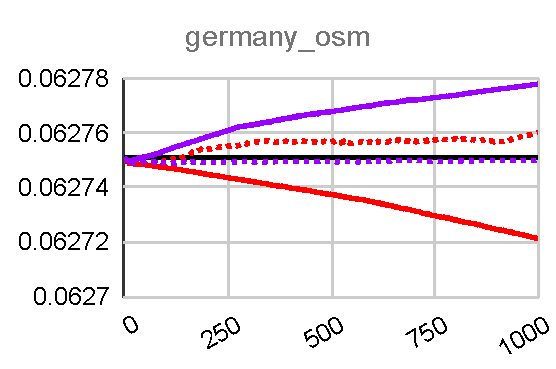
\includegraphics[width=0.23\linewidth]{out/im-germany_osm.pdf}
  }
  \subfigure{
    \label{fig:im-asia_osm}
    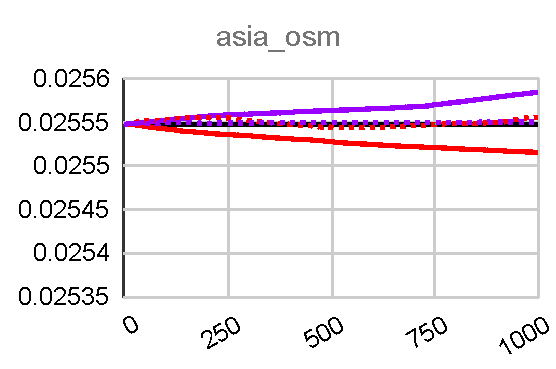
\includegraphics[width=0.23\linewidth]{out/im-asia_osm.pdf}
  }
  \subfigure{
    \label{fig:im-indochina-2004}
    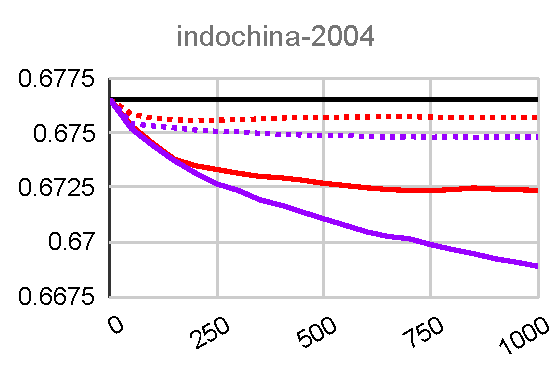
\includegraphics[width=0.23\linewidth]{out/im-indochina-2004.pdf}
  } \\[-2ex]
  \caption{Variation of Gini coefficient (Y-axis) with edges being added (X-axis) to the graphs incrementally with six different heuristics: \textit{edgeInsertCxrx}, \textit{edgeInsertCxSx}, \textit{edgeInsertCxSr}, \textit{edgeInsertCRrx}, \textit{edgeInsertCRSx}, and \textit{edgeInsertCRSr}.}
  \label{fig:im-all}
\end{figure*}

